\chapter{Begriffliche Grundlagen}

\section{Latent Dirichlet Allocation}
\todo[inline]{Herr Möhrle hat gesagt bei längeren Zitaten, Verweis nach dem ersten Satz}
\todo[inline]{Bei Erstverwendung einer Abkürzung (ABK) in Klammern?}
Die \acl{lda} (\ac{lda}) ist ein generatives Wahrscheinlichkeitsmodell für Textdokumente. \parencite[vgl.][S. 996]{Blei03latentdirichlet} Dokumente werden als zufällige Mischverteilungen über latente Themen dargestellt, wobei jedes Thema eine Wahrscheinlichkeitsverteilung über Worte ist. 

Vereinfacht gesagt werden alle Dokumente mit einer Wahrscheinlichkeit zu vorher unbekannten Themen zugeordnet. Die Themen werden also durch den Algorithmus gefunden. Ein Thema besteht aus der Menge aller in den Dokumenten vorkommenden Wörtern und ihrer Wahrscheinlichkeit das sie zu diesem Thema gehören.
\todo{zitat finden}
Die Reihenfolge der Dokumente ist nicht relevant. Auch die Reihenfolge der Wörter in den Dokumenten wird nicht beachtet, sondern nur die Häufigkeit, es gilt das \acl{bow} Modell. \parencite[vgl.][S. 155-156]{harris1954distributional} Die Anzahl der latenten Themen muss vorher gegeben sein.
\todo{beispiel geben zu LDA}
Um die Anzahl an versteckten Themen zu approximieren werden alle \ac{lda} Modelle mit den Themenanzahlen von 1 bis 100 erstellt. Diese Modelle werden anhand ihrer Kohärenz innerhalb der Themen und anhand ihrer Distanz zwischen den Themen verglichen. Mithilfe dieser Daten sucht man ein Modell aus, das eine möglichst geringe Themenanzahl, hohe Kohärenz und hohe Distanz aufweist. Die Themenanzahl sollte möglichst gering sein, weil es aufwändig ist diese Themen zu interpretieren und die Distanz bei zu hoher Themenzahl sinkt.

\begin{figure}[htpb]
	\centering
	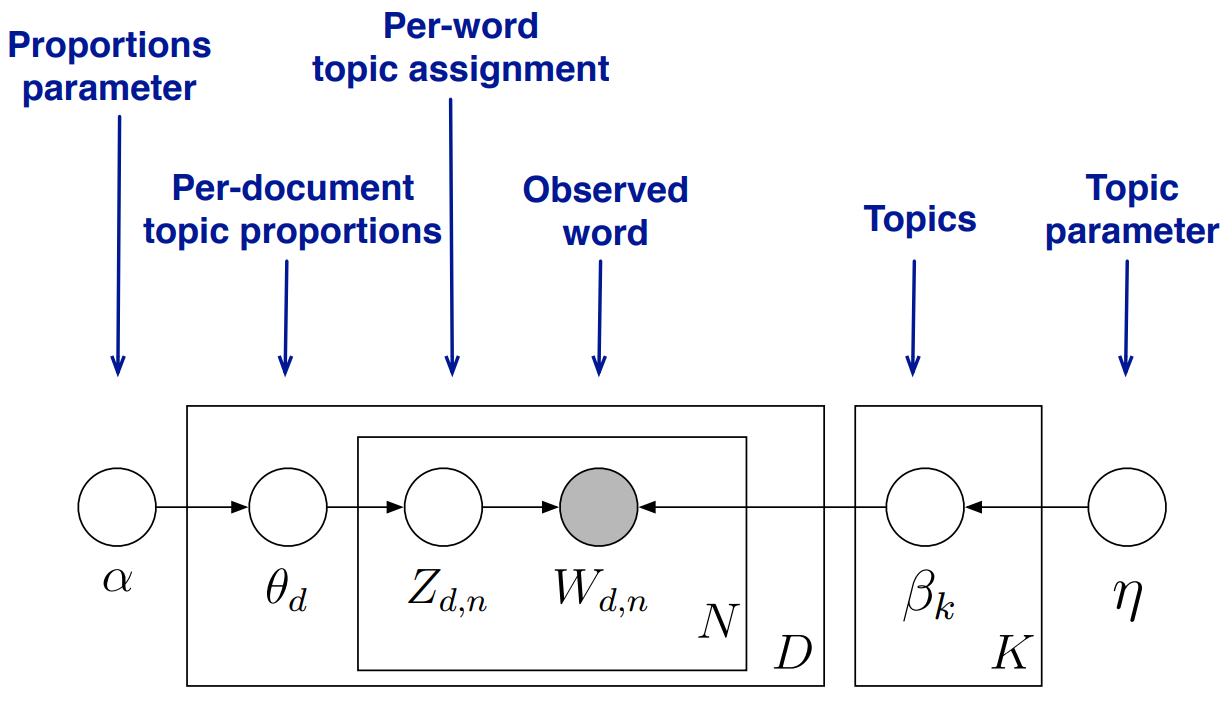
\includegraphics[width=\textwidth,height=8cm,keepaspectratio=true]{lda.png}
	\caption{
		LDA als graphisches Modell, von \parencite[vgl.][S. 23]{ProbabilisticTopicModels}
	}
	\label{fig:LDA Modell}
\end{figure}


$\mathcal{W}$ ist das Wort aus $\mathcal{N}$ Wörtern eines Dokuments i. Dieses Dokument i ist eines aus allen Dokumenten $\mathcal{M}$. Alle folgenden Parameter sind latent. $\mathcal{Z}$ ist das Thema für das Wort j aus besagtem Dokument i. Jedem Wort wird ein Thema zugeordnet. Wodurch jedes Dokument eine Mischung aus allen Themen ist. Die Verteilung der Themen für Dokument i ist $\theta$. Die Hyperparameter $\alpha$ und $\beta$ der \acl{lda}. $\alpha$ bestimmt die Dokument-Themen Verteilung und die Wort-Themen Verteilung. Ein hoher $\alpha$ Wert erhöht die Wahrscheinlichkeit dafür das einem Dokument mehr Themen zugeordnet werden. Ein niedriger $\alpha$ Wert verringert die Wahrscheinlichkeit das einem Dokument mehrere Themen zugeordnet werden. Ein hoher $\beta$ Wert erhöht die Wahrscheinlichkeit das einem Thema mehr Wörter zugeordnet werden. Ein niedriger $\beta$ Wert erhöht die Wahrscheinlichkeit das einem Thema weniger Wörter zugeordnet werden. Vereinfacht gesagt lässt ein großer $\alpha$ Wert die Dokumente ähnlicher aussehen und ein hoher $\beta$ Wert lässt die Themen ähnlicher aussehen. Mit diesem Algorithmus lässt sich ein Model erstellen, das jedes Wort mit Wahrscheinlichkeit zu jedem Thema zuordnet.

\begin{figure}[htpb]
	\centering
	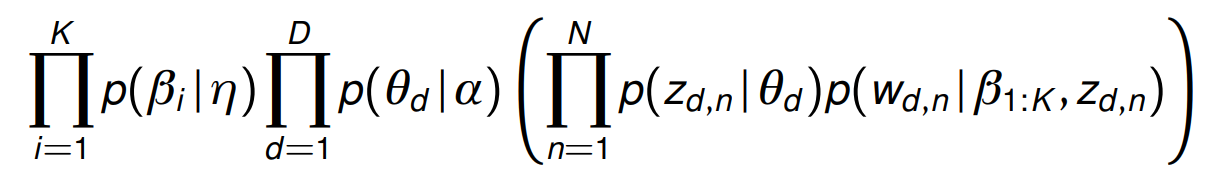
\includegraphics[width=\textwidth,height=3cm,keepaspectratio=true]{ldaDocLikelyhood.png}
	\caption{
		LDA als graphisches Modell, von \parencite[vgl.][S. 25]{ProbabilisticTopicModels}
	}
	\label{fig:LDA Formel}
\end{figure}


Dies ist die Wahrscheinlichkeit ein Dokument zu generieren, mit den Einstellungen des \ac{lda} Modells. Die Wahrscheinlichkeit ist gering aber je höher sie ist desto besser ist das Modell. Die vier Komponenten der Formel sind die Einstellungen des \ac{lda} Modells als Faktoren. Diese ergeben wiederum eigene Wahrscheinlichkeiten. Der Erste Faktor ist eine Dirichletverteilung von Dokumenten zu Themen. Eine Dirichletverteilung kann man sich als n-Simplex vorstellen, mit n gleich der Anzahl von Themen. Jedes Dokument hat eine Wahrscheinlichkeit für die Zugehörigkeit zu jedem Thema. Die Dirichletverteilung ist also eine Verteilung von Verteilungen. Der zweite Faktor ist eine Dirichletverteilung von Themen zu Wörtern und verhält sich analog zur ersten.

Der dritte Faktor ist eine Multinomialverteilung des ersten Faktors. Eine Multinomialverteilung ist wie eine Urne mit mehreren verschiedenen Themen, die mit Wahrscheinlichkeiten gezogen werden können. Diese zweite Multinomialverteilung ist also eine von Themen. Der Vierte Faktor ist eine Multinomialverteilung des zweiten Faktors mit Worten. Diese verhält sich analog zur ersten.

Kombiniert man diese Multinomialverteilungen miteinander, indem man immer ein Thema aus der ersten zieht und zu dem Thema passend ein Wort aus der zweiten, generiert man ein neues Dokument. Dies wird wiederholt bis gleich viele Dokumente generiert wurden wie verarbeitet wurden. Die Wahrscheinlichkeit das man mit dieser Methode die gleichen Dokumente erzeugt ist wie gesagt gering.

Die Dirichletverteilungen werden mit den $\alpha$ und $\beta$ Werten beeinflusst. Es werden viele verschiedene Werte getestet und das Modell mit der höchsten Wahrscheinlichkeit die gleichen original Dokumente zu erzeugen gewinnt.



\todo{warum LDA? in der conclusion: stevens2012exploring}



\section{Dynamic Latent Dirichlet Allocation}
Die \acl{dlda} (\ac{dlda}) ist eine Version des \ac{lda}, welche die chronologische Reihenfolge der Dokumente berücksichtigt. Dadurch ist es möglich die Veränderung der Themenschwerpunkte über den Zeitraum zu betrachten. \parencite[vgl.][]{dynamicLDA}

\section{Hierarchical Latent Dirichlet Allocation}
Hierarchisches \ac{lda} (\ac{hlda}) erweitert \ac{lda}, um eine beliebig tiefe  Hierarchie aus Unterthemen. \parencite[vgl.][]{griffiths2004hierarchical} Diese lassen sich als Baumdiagramm darstellen. Dadurch erhält man noch mehr Informationen zu einem Thema, um es genauer zu benennen. Auch Cluster lassen sich dadurch erkennen. \ac{hlda} benutzt den \acl{crp} (\ac{crp}). Angenommen es gibt ein chinesisches Restaurant mit unendlich vielen Tischen, an denen unendlich viele Gäste sitzen können. Der erste Gast setzt sich an den ersten Tisch. Der zweite Gast setzt sich an den ersten Tisch mit der Wahrscheinlichkeit () und an einen unbesetzten Tisch mit der Wahrscheinlichkeit (). 

\section{Hierarchical Dirichlet Process}